\documentclass[12pt]{article}

% refer to configurations.tex for the LaTeX setup of this template
\usepackage[english]{babel}

\title{\textbf{\textsf{Tauola \\}}}
\date{\today}
\author{}

% math
\usepackage{amsmath, amssymb}

% references
\usepackage[style=apa, backend=biber]{biblatex}
\addbibresource{bibliography.bib}

% fonts
%\usepackage{helvet}
%\usepackage{sectsty}
%\allsectionsfont{\sffamily} % for section titltes use sans-serif
% \renewcommand{\familydefault}{\sfdefault} % comment out for sans-serif font
% \usepackage{sansmath} % comment out for sans-serif math font
% \sansmath % comment out for sans-serif math font

% margins
\usepackage{geometry}
\geometry{
  a4paper,
  total={170mm,257mm},
  left=25mm,
  right=25mm,
  top=30mm,
  bottom=30mm,
}

% no indentation when a new paragraph starts
\setlength{\parindent}{0cm}

% links
\usepackage{hyperref} % better links
\usepackage{color}    % nicer link colors
\definecolor{pigment}{rgb}{0.2, 0.2, 0.6}
\hypersetup{
  colorlinks = true, % Color links instead of ugly boxes
  urlcolor   = pigment, % Color for external hyperlinks
  linkcolor  = black, % Color for internal links
  citecolor  = pigment % Color for citations
}

\usepackage{graphicx}

%here is the path
\graphicspath{ {./images/} }

% headers
\usepackage{fancyhdr}
\pagestyle{fancy}
\lhead{Tauola}
\chead{}
\rhead{}

% example boxes
\usepackage{tcolorbox}
\newtcolorbox{examplebox}{
  colback=white,
  colframe=gray!30,
  title=Example,
  sharp corners,
  boxrule=0.5pt,
  coltitle=black
}

%bash script
\usepackage{minted}


% conditionals
\usepackage{ifthen}
\newboolean{showinstructions}
\newboolean{showexamples}
\newboolean{showexplanations}
\renewenvironment{examplebox}{%
  \ifthenelse{\boolean{showexamples}}%
    {\begin{tcolorbox}[colback=white, colframe=gray!30, title=Example, sharp corners, boxrule=0.5pt, coltitle=black]}%
    {\expandafter\comment}%
}{%
  \ifthenelse{\boolean{showexamples}}%
    {\end{tcolorbox}}%
    {\expandafter\endcomment}%
}

% Define a new environment for explanations
\newcommand{\explanation}[1]{%
  \ifthenelse{\boolean{showexplanations}}%
    {\textit{Explanation:} #1}%
    {\ignorespaces}%
}

% Define a new environment for instructions
\newcommand{\instructions}[1]{%
  \ifthenelse{\boolean{showinstructions}}%
    {#1}%
    {\ignorespaces}%
}

\makeatletter
\newcommand{\maketitlepage}{%
    \begin{titlepage}
        \maketitle
        \thispagestyle{empty}
        \vfill 
        \centering
        Version: 1.1.8 \\
        Last updated: 2025-03-02 \\
        Report based on the source code and papers:\\
    \url{https://tauolapp.web.cern.ch/resources/TAUOLA.1.1.8/Tauola_interface_design.1.1.8.pdf}, 
        \vfill 
    \end{titlepage}
    \newpage
}
\makeatother

% Optional user settings
\setboolean{showinstructions}{true} % set to false to hide instructions
\setboolean{showexamples}{true} % set to false to hide examples
\setboolean{showexplanations}{true} % set to false to hide explanations

\begin{document}
\maketitlepage

\section{Installation}

For Tauola installation, you need the HepMC2 and HepMC3.\\

For HepMC2 and HepMC3 package, you download the source code and create a build directory. Then run the following command from the build directory.

\begin{minted}{bash}
cmake -DCMAKE_INSTALL_PREFIX=/home/john/products/HepMC2/HepMC-2.06.11/ 
/home/john/products/HepMC2/HepMC-2.06.11/ -Dmomentum:STRING=GEV
-Dlength:STRING=MM 
\end{minted}

For the installation of Tauola, you can do 
\begin{minted}{bash}
./configure --prefix=/home/john/products/Tauola/TAUOLA 
--with-hepmc=/home/john/products/HepMC2/HepMC-2.06.11/ 
--with-hepmc3=/home/john/products/HepMC3/HepMC3-3.3.0 
--with-lhapdf=/home/john/products/LHAPDF/LHAPDF-6.5.5 
--with-pythia8=/home/john/products/Pythia8/pythia8313 
--with-mc-tester=/home/john/products/MC-TESTER/mc-tester
\end{minted}


\section{Tauola Subroutines}
\subsection{JAKER}
\textbf{SUBROUTINE JAKER(JAK)}\\
This subroutine selects the decay modes depending on the branching ratio. JAK is an integer that determines which tau decay mode is selected. Each JAK value corresponds to a specific decay channel (e.g., tau → electron + neutrinos).

\begin{itemize}
    \item JAK=0 - Allows according to standard model
    \item JAK=1 - electron mode ($\tau \rightarrow  e \nu_\tau \nu_e$)
    \item JAK=2 - muon mode ($\tau \rightarrow  \mu \nu_\tau \nu_\mu$)
    \item JAK=3 - pion mode ($\tau \rightarrow  \pi \nu_\tau$)
    \item JAK=4 - rho mode ($\tau \rightarrow  \rho \nu_\tau$)
    \item JAK=5 - A1 mode (axial-vector meson)($\tau \rightarrow  a1 \nu_\tau$)
    \item JAK=6 - K mode ($\tau \rightarrow  K \nu_\tau$)
    \item JAK=7 - K* mode ($\tau \rightarrow  K* \nu_\tau$)
    \item JAK=8 - n$\pi$ mode ($\tau \rightarrow  n\pi \nu_\tau$)
\end{itemize}

\subsubsection{global variables}
{\textbf{Taubra}\\
GAMPRT(30) - The partial widths (branching probabilities) of different decay modes.\\
JLIST(30) - The list of decay mode identifiers.\\
NCHAN - The number of possible decay channels.\\}

\subsubsection{local variables}
{CUMUL(30) - Stores cumulative sums of branching ratios.\\
RRR(1) - Stores a random number used for selection.\\
}\\
It ensures number of decay channels is within the valid range. If NCHAN is less than 1 or greater than 30, the program exits with an error.\\

Suppose mode 1 has 30$\%$, mode 2 has 50$\%$ and mode 3 has 20$\%$ probability, the cummuliative array will be 30, 80,100 $\%$ probabilities respectively. Then it iterate through the list of decay channel and if the random number (0,1) falles within the range, that particular decay mode is selected. The branching ratios are not filled in this subroutine\\

The decay mode identifier in JLIST is passed to JAK variable

\subsection{DEKAY}
\textbf{SUBROUTINE DEKAY(KTO,HX)}\\
This subroutine handles the decay of tau leptons, including initialization, decay mode selection, and final state transformations. \\

The IF statement and its ELSEIF branches control the program's behavior based on KTO

KTO = -1  - Initialization
KTO = 1   - $\tau^+$ decay
KTO = 2   - $\tau^-$ decay
KTO = 11  - Completing $\tau^+$ decay
KTO = 12  - Completing $\tau^-$ decay
KTO = 100 - Final Processing



\subsubsection{global variables}
\textbf{JAKI}\\
JAK1 - \\
JAK2 - \\
JAKP - \\
JAKM - \\
KTOM - \\

\textbf{IDFC}\\
IDF - \\

\textbf{TAUPOS}\\
NP1 - \\
NP2 - \\

\textbf{TAUBMC} \\
GAMPMC(30) - \\
GAMPER(30) - \\
NEVDEC(30) - \\

\textbf{TAUDCD} \\
IDFFIN(9,NMODE) -  2D array\\
MULPIK(NMODE) - \\
NAMES(NMODE)*31 - Character array\\

\textbf{INOUT}\\
INUT - \\
IOUT - \\

\subsubsection{local variables}

H(4) - temporaryily used\\
HX(4) (double) - A polarimetric vector used by the host program for calculating the spin weight of tau decay\\
GAMPMC(double) - \\
GAMPER(double) - \\
PDUM1(4),PDUM2(4),PDUM3(4),PDUM4(4),PDUM5(4) - \\
HDUM(4) - \\
PDUMX(4,9) - \\
IWARM = 0\\

\subsubsection{Constants}

NMODE=15   - Likely represents the number of decay modes available in the subroutine\\
NM1=0, NM2=1, NM3=8, NM4=2, NM5=1, NM6=3




\subsection{DADNEW}
\textbf{SUBROUTINE DADNEW(MODE,ISGN,HV,PNU,PWB,PNPI,JNPI)}\\
NMODE = 196 - Total number of decay modes handled in this subroutine.


\subsubsection{global variables}
\textbf{PARMAS}\\
This block stores masses and decay widths of fundamental particles, mainly mesons and leptons, used in the tau decay simulation.\\
AMTAU  - Mass of the $\tau$ lepton\\
AMNUTA - Mass of the $\tau_\nu$\\
AMEL   - Mass of electron\\
AMNUE  - Mass of $\nu_e$\\
AMMU   - Mass of $\mu^-$\\
AMNUMU - Mass of $\nu_\mu$\\
AMPIZ  - Mass of $\pi^0$\\
AMPI   - Mass of $\pi^-$\\
AMRO   - Mass of $\rho$ meson\\
GAMRO  - Decay width of $\rho$ meson\\
AMA1   - Mass of $A_1$ meson\\
GAMA1  - Decay width of $A_1$ meson\\
AMK    - Mass of charged Kaon\\
AMKZ   - Mass of K$^0$\\
AMKST  - Mass of K$^*$ meson\\
GAMKST - Decay width of K$^*$ meson\\


\textbf{DECPAR}\\
GFERMI - Fermi's constant $G_F$\\
GV     - Vector coupling constant for weak interactions\\
GA     - Axial-vector coupling constant\\
CCABIB - Cosine of the Cabibbo angle cos($\theta_c$), governing quark mixing in weak decays\\
SCABIB - Sine of the Cabibbo angle cos($\theta_c$), also related to quark mixing\\
GAMEL  - Partial decay width of the electron decay channel ($\tau \rightarrow e \nu_e \tau$ )\\

CCABIB and SCABIB determine decay rates involving Cabibbo-favored and Cabibbo-suppressed processes.\\

\textbf{TAUBMC}\\
GAMPMC(500)	- Stores the normalized partial decay widths for different tau decay channels\\
GAMPER(500) - Stores the uncertainty (error) in the decay widths\\
NEVDEC(500) - Stores the number of decays simulated for each channel\\

\textbf{TAUDCD}   -   Tau decay information\\
IDFFIN(9,NMODE)  - Likely represents the final-state particle IDs for each tau decay mode. 9 rows suggest that up to 9 particles can be tracked per decay mode.\\
MULPIK(NMODE) - Likely stores the multiplicity of pions ($\pi$) in each decay mode.\\
NAMES(NMODE)   - Stores the names of the decay channels.

\subsubsection{local variables}

PNU(4) - Four momentum of neutrino.\\
PWB(4) - Four vector of a particle in decay process.\\
PNPI(4,9) - Stores four-momentum components of up to 9 pions in a decay mode.\\
HV(4) - Stores a four-momentum used in computations.\\
HHV(4) - Possibly an intermediate calculation of HV(4), used for handling helicities or boosting frames.\\
PDUM1(4), PDUM2(4), PDUMI(4,9) - Dummy four-momentum variables used in calculations.\\

RRR(3) - Random number\\
WTMAX(NMODE) - Stores the maximum weight for each of the tau decay modes\\
SWT(NMODE) - Sum of weights for accepted events per decay mode.\\
SSWT(NMODE) - Sum of squared weights (used for error estimation).\\
NEVRAW(NMODE) - Total number of simulated decays per mode.\\
NEVOVR(NMODE) - Number of overweighted events per mode.\\
NEVACC(NMODE) - Number of accepted decays per mode.\\


\textbf{MODE=-1}  - triggers a specific initialization routine.\\
IWARM = 1 -  Marks the initialization as done.


What is Ntrials do? The 4$\pi$ phase space needs lot more trials at initialization (probably mentioning the number of samples), 

The initialization calls different decay phase space functions (DPH4PI, DPH5PI, etc.). This is probably to establish weights. Each function likely simulates a different multi-pion decay mode. The thresholds (NM4, NM5, etc.) define how many decay modes fall into each category.\\

\vspace{0.5cm}
\textbf{MODE=0} generates the tau decays based on initialized parameters.\\
Calls decay functions (DPH4PI, DPH5PI, etc.), but now actually records events.

Rotation transformations to align with tau rest frame.\\

The $\theta$ and $\phi$ is generated randomly across a sphere. \\

The ROTOR2 subroutine rotates PNU along y-axis THET units.\\
And ROTOR3 subroutine rotates PNU along z-axis PHI units.\\

It rotates, neutrino, W-boson and Some helicity or spin-related quantity randomly and isotropically.

\vspace{0.5cm}
\textbf{MODE=1} performs statistical calculations related to decay events and prints out results.



\subsubsection{DPH1PI}
\textbf{SUBROUTINE DPH1PI(WT,HV,PNU,PWB,PNPI,JNPI)}\\

This subroutine model the decay of tau lepton($\tau$) into a neutrino and a single meson. This subroutine computes the momentum of the decay products when a tau lepton ($\tau$) decays into a neutrino and a single meson.

Following are the masses used in tau decays \\
C IN-COMING / OUT-GOING  FERMION MASSES\\
      AMTAU  = 1.7842\\
C --- let us update tau mass ...\\
      AMTAU(m$_\tau$)        = 1.777\\
      AMNUTA(m$_{\nu_\tau}$) = 0.0 $!$ 0.010   (nearly zero(0 or $\leq$0.01))\\
      AMEL(m$_{e^-}$)        = 0.0005111\\
      AMNUE(m$_{\nu_e}$)     = 0.0\\
      AMMU(m$_\mu$)          = 0.105659 \\
      AMNUMU(m$_{\nu_\mu}$)  = 0.0\\
*\\
* MASSES USED IN TAU DECAYS\\
\\
      AMPIZ(m$_{\pi_0}$)     = 0.134976\\
      AMPI(m$_\pi$)          = 0.139570\\
      AMRO(m$_\rho$)         = 0.77590\\
      GAMRO($\Gamma_\rho$)   = 0.14790\\
*C    GAMRO                  = 0.666\\
      AMA1(m$_{a1}$)         = 1.251\\
      GAMA1($\Gamma_{a1}$)   = 0.599\\
      AMK(m$_K$)             = 0.493677\\
      AMKZ(m$_{K^0}$)        = 0.497672\\
      AMKST(m$_{K^*}$)       = 0.89166\\
      GAMKST($\Gamma_{K^*}$) = 0.0508\\

Some initilization - \\

(NLT=2,NMODE=196,NM1=40,NM2=71,NM3=19,NM4=32,NM5=21,NM6=13)\\

Here INUM determines the specific decay process. 

Using relativistic kinematics, the energy ($E_{KK}$,$E_\nu$) and momentum X$_{KK}$ of the meson and neutrino are given by:\\
\[E_{KK} = \frac{m_\tau^2+m_{KK}^2-m_\nu^2}{2m_\tau}\]

\[E_{\nu} = \frac{m_\tau^2-m_{KK}^2+m_\nu^2}{2m_\tau}\]

\[X_{KK} = \sqrt{E_{KK}^2-m_{KK}^2}\]

SPHERA(XKK, PKK) - Generates a random isotropic direction for the 3-momentum of the meson.\\
PKK(4) = EKK - Assigns the energy component of the meson's 4-momentum.\\
The neutrino’s 3-momentum(PNU) is the opposite of the meson's 3-momentum \\

\subsection{DAM1PI}
\textbf{SUBROUTINE DAM1PI(INUM,PNU,AMF0,PKK,AMF1,GAMM,HV)} - Line No : 3317\\

INUM - Decay channel identifier (1 for $\pi^- \nu_\tau$, 2 for $K^-\nu_\tau$)\\
PNU(4) - 4-momentum of neutrino\\
AMF0 - Mass of neutrino\\
PKK(4) - 4-momentum of the meson\\
AMF1 - Mass of the meson\\
GAMM - The decay width($\Gamma$)\\
HV(4) - \\

The decay parameters and the particle masses are loaded

The DAM1PI subroutine is responsible for computing the decay width ($\Gamma$) and angular distribution for the decay of a tau lepton ($\tau$) into a single pseudoscalar meson ($\pi$ or $K$) and a neutrino ($\nu_\tau$).\\


PXQ = AMTAU*EKK . Its just the scalar product of four momentum of tau and the meson($P_{\tau}$ $\cdot$ $P_{KK}$ = m$_\tau \cdot E_{KK}$). This is because the $\tau$ momentum is zero in $\tau$'s rest frame.\\

PXN=AMTAU*ENU. Similarly for $\nu_\tau$ also the ($P_{\tau}$ $\cdot$ $P_{\nu}$ = m$_\tau \cdot E_\nu$)\\

QXN = $P_{KK} \cdot P_\nu$ = $E_{KK}E_\nu - p_{KK} \cdot p_\nu$\\

\[BRAK = (G_V^2+G_A^2)(2P_\tau \cdot P_{KK} \cdot P_{KK} \cdot P_\nu - m_{KK}^2 P_\tau \cdot P_\nu)\ + (G_V^2 - G_A^2) m_\tau m_\nu m_{KK}^2 \]

The helicity vector HV determines the angular dependence of the decay.

\[ HV(1-3) = \frac{2G_AG_Vm_\tau (2p_{KK}(I) \cdot P_{KK} \cdot P_\nu - p_\nu(I) m_{KK}^2)}{BRAK}  \]

\[HV(4) = 1 \]

The decay width for the 2-body decay including the phase space factor.\\

INUM = 1 for $\tau^- \rightarrow \pi^- \nu_\tau$\\
INUM = 2 for $\tau^- \rightarrow K^- \nu_\tau$\\

\[\Gamma = \frac{G_F^2 f^2}{16\pi}m_\tau^3\Big(\frac{BRAK}{m_\tau^4}\Big)\sqrt{\frac{(m_\tau^2-m_{KK}^2-m_\nu^2)^2-4m_{KK}^2m_\nu^2}{m_\tau^4}}\]

f is the pion/kaon decay constant ($f_\pi$= 0.1284 and $f_{K} = 0.0354$)\\

The last part of the subroutine is made as a placeholder for the potential non-standard model modification's such as
\begin{itemize}
    \item Matrix element corrections
    \item Dalitz plot effects
    \item Other beyond-SM physics contributions
\end{itemize}

IME values\\
\begin{itemize}
    \item IME=2 decay into pion/kaon + neutrino
    \item IME=4 Another decay mode with decay constant $f$ computed externally 
    \item IME=5 Calls an external wrapper (DAM1PI\_wrap), possibly for beyond-SM physics
    \item IME=0 Not initialized, assigns default values
    \item IME=Others Assumes flat phase space (basic decay model)
\end{itemize}

\subsection{DPH4PI}
\textbf{SUBROUTINE DPH4PI(DGAMT,HV,PN,PAA,PMULT,JNPI)}-Line no 3411

This subroutine simulates the decay of A1 meson in the rest frame of the $\tau$ lepton, with $A_1$ momentum aligned along the z-axis. The decay process involves generating momenta for multiple particles, handling resonances, and computing the corresponding phase-space factors.

HV(4) - Helicity vector (4-momentum of the $a_1$) \\
PT(4) - 4-momentum of the $\tau$ lepton (initialized at rest)\\
PN(4) - 4-momentum of the $\nu_\tau$\\
PAA(4) - 4-momentum of the $a_1$ meson\\
PIM1(4), PIM2(4), PIPL(4) - 4-momenta of final state charged pions\\
PIZ(4) - 4-momentum of the neutral pion\\
PR(4) - Auxiliary momentum variable used for reference frame changes\\
PMULT(4,9) - Stores momenta of multiple decay products\\ \\

UU - Likely a parameter related to kinematic calculations, such as an invariant mass squared or a phase-space variable.\\
FF, FF1, FF2, FF3, FF4 - Jacobian correction factor.\\
GG1, GG2, GG3, GG4 - Use is not clear.\\
XLAM(X,Y,Z) - Computes the Källén function $\lambda(x,y,z)$.\\

PHSPAC - $\frac{1}{2^{23}\pi^{11}}$.\\ \\
PHSP - $\frac{1}{2^5 \pi^2}$ = $\frac{1}{32 \pi^2}$.\\ \\
AMP1, AMP2, AMP3, AMP4 - Masses of the final state particles.\\
AM4SQ, AM3SQ, AM2SQ - Squared masses of 4, 3, and 2-pion systems.\\
ALP1, ALP2, ALP - Angles for resonance sampling.\\
EXE - Boost factor for Lorentz transformations.\\

CHOICE4 - Chooses resonance parameters for phase space sampling.\\

PT is initialized with the $\tau$ lepton four momentum values at rest.\\

AMP1 - $\pi^-$  mass\\
AMP2 - Another $\pi^-$  mass\\
AMP3 - $\pi^+$  mass\\
AMP4 - $\pi^0$ mass

The $\tau$ might decay to some unstable particles and they decay to other particles. The mass of a resonance is not fixed, but follows a Breit-Wigner distribution characterized by a central mass $m_\rho$ and width $ \Gamma_\rho$.


\[AMS1 = m_\pi^2 = (m_{\pi1^-} + m_{\pi2^-} + m_{\pi1^+} + m_{\pi^0})^2\]

\[AMS2 = (m_\tau - m_{\nu_\tau})^2\]


\subsubsection{4-Pion System Mass (AM4)}

\[\frac{dN}{dm_\pi} = \frac{\Gamma_\rho}{(m_\pi^2 - m_\rho^2)^2 + (m_\rho \Gamma_\rho)^2} \]


This is implemented using the inverse transform sampling method.\\

To derive the CDF for the breit-wigner distribution, we need to integrate from ${-\infty}$ to $m_\pi^2$. 

\[F(m_\pi^2) = \int_{-\infty}^{m_\pi^2}  \frac{\Gamma_\rho}{(m_\pi^{'2} - m_\rho^2)^2 + (m_\rho \Gamma_\rho)^2}dm_\pi^{'2} \]

The integral has the standard form:
\[\int \frac{dx}{x^2+a^2} = \frac{1}{a}tan^{-1}\Big(\frac{x}{a}\Big)\]

where we define 
\[x = m_\pi^{'2} - m_\rho^2,   \;\;\; a = m_\rho \Gamma_\rho \]

\[dx = dm_\pi^{'2}\]

This substitution transforms our integral into:

\[F(m_\pi^2) = \int_{-\infty}^{m_\pi^2-m_\rho^2}  \frac{\Gamma_\rho}{x^2 + (m_\rho \Gamma_\rho)^2}dx\]
%\frac{dx}{2\sqrt{x+m_\rho^2}} \]

Applying the standard integral formula:

\[F(m_\pi^2) = \frac{1}{m_\rho \Gamma_\rho} \Bigg[ \frac{\pi}{2} + tan^{-1}\Big( \frac{m_\pi^2-m_\rho^2}{m_\rho \Gamma_\rho}\Big) \Bigg]\]

Now we have to invert the CDF for sampling,

\[F(m_\pi^2) = U\]

where U is the uniform random number form [0,1] and solve for $m_\pi^2$

\[Um_\rho \Gamma_\rho - \frac{\pi}{2} = tan^{-1}\Bigg( \frac{m_\pi^2-m_\rho^2}{m_\rho \Gamma_\rho} \Bigg)\]

\[tan (Um_\rho \Gamma_\rho - \frac{\pi}{2}) = \frac{m_\pi^2-m_\rho^2}{m_\rho \Gamma_\rho}\]

Solving for $m_\pi^2$,
\[m_\pi^2 =  m_\rho^2 + m_\rho \Gamma_\rho tan(Um_\rho \Gamma_\rho - \frac{\pi}{2})\]


From the code its,

\[ ALP1 = tan^{-1}\Big(\frac{m_\pi^2- m_\rho^2}{m\rho \Gamma_\rho}\Big)\]


\[ALP2 = tan^{-1}\Big(\frac{(m_\tau - m_{\nu_\tau})^2- m_\rho^2}{m\rho \Gamma_\rho}\Big)\]

\[ALP = ALP1+ U(ALP2-ALP1)\]

\[m_\pi^2 =  m_\rho^2 + m_\rho \Gamma_\rho tan(ALP)\]

Has to see how the difference arise........................\\

\vspace{1cm}

THREE BODY PHASE SPACE NORMALIZED AS IN BJORKEN-DRELL\\

The phase space weight PHSPAC is updated based on this resonance shape.

\[PHSPAC = \frac{1}{2^{23}\pi^{11}}\Big( \frac{(m_\pi^2-m_\rho^2)^2+ (m\rho \Gamma_\rho)^2}{m_\rho \Gamma_\rho}\Big) \times (ALP2-ALP1)\]


%\\The jacobian mentioned in the code refers to the Jacobian factor used to adjust for the phase space volume element in a Monte Carlo simulation of particle decays. The Jacobian is essential when transforming from one set of variables (e.g., the initial particle momenta or energies) to another (e.g., the momenta or energies of the decay products in the final state).

\subsubsection{3-Pion System Mass (AM3)}

The program determines whether to use a flat phase space sampling or include another resonance (like $\omega$). $\omega$ is sampled in the three pion system with a narrower Breit-Wigner shape. \\

If a second random number RRR(9) is greater than a threshold (PREZ), a flat phase space model is used:

\[m_{3\pi}^2 = ( m_{\pi2^-} + m_{\pi1^+} + m_{\pi^0})^2 + U* \Big((m_\pi - m_{\pi1^-})^2 - ( m_{\pi2^-} + m_{\pi1^+} + m_{\pi^0})^2\Big)\]


Note that one pion is less\\

Otherwise, a Breit-Wigner sampling for the omega meson ($\omega$) is applied, using a method similar to the $\rho$ resonance treatment above.\\

Jacobian factor FF1, if its flat phase space is

\[FF1 = (m_\pi - m_{\pi1^-})^2 - ( m_{\pi2^-} + m_{\pi1^+} + m_{\pi^0})^2\]

If its Breit-Wigner, 

\[FF1 = \frac{(m_{3\pi}^2 -m_\omega^2)^2 + (m_\omega \Gamma_\omega)^2}{m_\omega \Gamma_\omega} \times (ALP2-ALP1)\]

\subsubsection{2-Pion System Mass (AM2)}

A similar method is applied for the two-pion invariant mass.\\
It uses flat phase space sampling.

The Jacobian term for this is stored in FF2

\subsubsection{Final 2-Pion Kinematics in the Rest Frame}
The program computes the energies of two final-state pions in the rest frame:

\[E_{\pi^+} = \frac{m_{2\pi}^2- m_{\pi^+}^2+m_{\pi^0}^2}{2m_{2\pi}}\]
\[E_{\pi^0} = \frac{m_{2\pi}^2+ m_{\pi^+}^2-m_{\pi^0}^2}{2m_{2\pi}}\]

\[p_{\pi^0} = \sqrt{E_{\pi^0}^2 - m_{\pi^0}^2}\]

\[PHSPAC = PHSPAC \times 4\pi \times (\frac{2 p_{\pi^0}}{m_{2\pi}}) \]

The SPHERA subroutine generates a random 3D vector uniformly distributed on a sphere of radius $p_{\pi^0}$ and returns to variable PIZ.\\

The $\pi^+$ momentum will be the negative of the $\pi^0$ in rest frame.\\



\subsubsection{Finding the 4-momentum of the intermediate particle}

PR is the momentum of the intermediate particle (2pi system). \\

\[PR(1) = 0\]
\[PR(2) = 0\]
\[PR(4) = E_{PR} = \frac{m_{3\pi}^2+m_{2\pi}^2- m_{\pi^-}^2}{2m_{3\pi}}\]
\[PR(3) = \sqrt{abs(E_{PR}^2-m_{2\pi}^2)} \]

PIM1 - momentum of the $\pi^-$ 

\[PIM1(1) = 0\]
\[PIM1(2) = 0\]
\[PIM1(4) = E_{\pi^-} = \frac{m_{3\pi}^2-m_{2\pi}^2+ m_{\pi^-}^2}{2m_{3\pi}}\]
\[PIM1(3) = -PR(3)\]

This following factor accounts for the Jacobian when transforming between momentum variables.
\[FF3 = 4\pi\frac{2 p_{z,2\pi}}{m_{3\pi}}\]


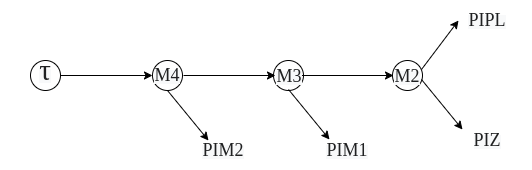
\includegraphics[width=14cm]{tauola_4pion.drawio.png}

\subsubsection{Boosting}

The BOSTER3(EXE,PVEC,QVEC) subroutine boost PVEC with EXE and outputs the boosted one in QVEC.

Here \[EXE = e^\eta, \;\;\;\;\; where \;\;\; \eta \;\; is \;\;  the \;\; hyperbolic \;\; velocity\]

\[e^\eta = cosh \eta + sinh \eta = \frac{E}{M}+\frac{p_z}{M}\]


\[EXE= e^\eta  = \frac{PR(4) +PR(3)}{m_{2\pi}}\]


Coming to the Boost subroutine

\[QVEC(4) = E^{'} =  \frac{(E+p_z)e^\eta + (E-p_z)e^{-\eta}}{2}\]

\[QVEC(3) = p_z^{'} =  \frac{(E+p_z)e^\eta - (E-p_z)e^{-\eta}}{2}\]

	
We do the boosting to PIZ and PIPL to $m_{2\pi}$'s frame. Then we apply random rotation to PIPL, PIM1, PIZ and $m_{2\pi}$.\\

Then we will solve for the four vector of $m_{3\pi}$ and PIM2. \\

Later we will again boost PIZ, PIPL, PIM1 to $m_{3\pi}$'s frame. Then we will apply random rotation to PIPL, PIM1, PIM2, PIZ and $m_{3\pi}$\\

The last step is finding $m_{4\pi}$ four momentum(PAA) and the neutrino four momentum(PN).\\

There is no boosting done on this. \\

There is a swapping of PIM1 and PIM2 momentum for a small fraction of events. The reason is 
not clear to me at this time. It's mentioned in the code as a bug fix.


The jacobian factors calculated earlier are not used. They are recalculated in the following sections.

\subsubsection{Flat Phase Space Channel}
Recalculate the $m_{3\pi}$ from the calculated momentum of the three pions.

\[m_{3\pi}^2 = AM3SQ \]
\[= (E_{\pi^-}+E_{\pi^+}+E_{\pi^0})^2 - (pz_{\pi^-}+pz_{\pi^+}+pz_{\pi^0})^2- (py_{\pi^-}+py_{\pi^+}+py_{\pi^0})^2- (px_{\pi^-}+px_{\pi^+}+px_{\pi^0})^2\]

\[AMS1 = (m_{\pi2^-} + m_{\pi^+} + m_{\pi^0})^2\]
\[AMS2 = (m_{4\pi}-m_{\pi^-})^2\]

\[FF1 = AMS2 - AMS1\]

\[AMS1 = (m_{\pi1^+} + m_{\pi^0})^2\]
\[AMS2 = (m_{3\pi}-m_{\pi2^-})^2\]


\[FF2=AMS2-AMS1\]

\[FF3 =  4\pi \frac{\lambda^{1/2}(m_{3\pi}^2, m_{2\pi}^2, m_{\pi2^-}^2)}{m_{3\pi}^2}\]

\[FF4 =  4\pi \frac{\lambda^{1/2}(m_{4\pi}^2, m_{3\pi}^2, m_{\pi1^-}^2)}{m_{4\pi}^2}\]

\[UU = FF1 \times FF2 \times FF3 \times FF4\]

\[UU = \Big((m_{4\pi}-m_{\pi^-})^2 - (m_{\pi2^-} + m_{\pi1^+} + m_{\pi^0})^2\Big) \times
	\Big( (m_{3\pi}-m_{\pi^-})^2 - (m_{\pi^+} + m_{\pi^0})^2\Big)  \]
	\[\times 4\pi \frac{\lambda^{1/2}(m_{3\pi}^2, m_{2\pi}^2, m_{\pi^-}^2)}{m_{3\pi}^2} \times
	4\pi \frac{\lambda^{1/2}(m_{4\pi}^2, m_{3\pi}^2, m_{\pi^-}^2)}{m_{4\pi}^2} \]


\subsubsection{Breit Wigner Phase Space Channel}

\[m_{3\pi}^2 = AM3SQ \]
\[= (E_{\pi^-}+E_{\pi^+}+E_{\pi^0})^2 - (pz_{\pi^-}+pz_{\pi^+}+pz_{\pi^0})^2- (py_{\pi^-}+py_{\pi^+}+py_{\pi^0})^2- (px_{\pi^-}+px_{\pi^+}+px_{\pi^0})^2\]

\[AMS1 = (m_{\pi2^-} + m_{\pi^+} + m_{\pi^0})^2\]
\[AMS2 = (m_{4\pi}-m_{\pi^-})^2\]

\[ALP1 = tan^{-1}\Big(\frac{(m_{\pi2^-} + m_{\pi^+} + m_{\pi^0})^2 - m_\rho^2}{m_\rho \Gamma_\rho}\Big)\]

\[ALP2 = tan^{-1}\Big(\frac{(m_{4\pi}-m_{\pi^-})^2 - m_\rho^2}{m_\rho \Gamma_\rho}\Big)\]


\[FF1 = \frac{(m_{3\pi}^2 - m_\rho^2)^2 + 	m_\rho^2 \Gamma_\rho^2}{m_\rho \Gamma_\rho} \times \Bigg(tan^{-1}\Big(\frac{(m_{4\pi}-m_{\pi^-})^2 - m_\rho^2}{m_\rho \Gamma_\rho}\Big) -  tan^{-1}\Big(\frac{(m_{\pi2^-} + m_{\pi^+} + m_{\pi^0})^2 - m_\rho^2}{m_\rho \Gamma_\rho}\Big)  \Bigg)\]


\[AMS1 = (m_{\pi1^+} + m_{\pi^0})^2\]
\[AMS2 = (m_{3\pi}-m_{\pi2^-})^2\]


\[FF2=AMS2-AMS1\]

\[FF3 =  4\pi \frac{\lambda^{1/2}(m_{3\pi}^2, m_{2\pi}^2, m_{\pi2^-}^2)}{m_{3\pi}^2}\]

\[FF4 =  4\pi \frac{\lambda^{1/2}(m_{4\pi}^2, m_{3\pi}^2, m_{\pi1^-}^2)}{m_{4\pi}^2}\]


\[FF = FF1 \times FF2 \times FF3 \times FF4\]


\subsubsection{Second Channel With Breit Wigner}

\[m_{3\pi}^2 = AM3SQ \]
\[= (E_{\pi2^{-}}+E_{\pi^+}+E_{\pi^0})^2 - (pz_{\pi2^{-}}+pz_{\pi^+}+pz_{\pi^0})^2- (py_{\pi2^-}+py_{\pi^+}+py_{\pi^0})^2- (px_{\pi2^-}+px_{\pi^+}+px_{\pi^0})^2\]

\[AMS1 = (m_{\pi1^-} + m_{\pi^+} + m_{\pi^0})^2\]
\[AMS2 = (m_{4\pi}-m_{\pi2^-})^2\]

\[ALP1 = tan^{-1}\Big(\frac{(m_{\pi1^-} + m_{\pi^+} + m_{\pi^0})^2 - m_\rho^2}{m_\rho \Gamma_\rho}\Big)\]

\[ALP2 = tan^{-1}\Big(\frac{(m_{4\pi}-m_{\pi2^-})^2 - m_\rho^2}{m_\rho \Gamma_\rho}\Big)\]


\[GG1 = \frac{(m_{3\pi}^2 - m_\rho^2)^2 + 	m_\rho^2 \Gamma_\rho^2}{m_\rho \Gamma_\rho} \times \Bigg(tan^{-1}\Big(\frac{(m_{4\pi}-m_{\pi2^-})^2 - m_\rho^2}{m_\rho \Gamma_\rho}\Big) -  tan^{-1}\Big(\frac{(m_{\pi1^-} + m_{\pi^+} + m_{\pi^0})^2 - m_\rho^2}{m_\rho \Gamma_\rho}\Big)  \Bigg)\]


\[AMS1 = (m_{\pi1^+} + m_{\pi^0})^2\]
\[AMS2 = (m_{3\pi}-m_{\pi1^-})^2\]


\[GG2=AMS2-AMS1\]

\[GG3 =  4\pi \frac{\lambda^{1/2}(m_{3\pi}^2, m_{2\pi}^2, m_{\pi1^-}^2)}{m_{3\pi}^2}\]

\[GG4 =  4\pi \frac{\lambda^{1/2}(m_{4\pi}^2, m_{3\pi}^2, m_{\pi2^-}^2)}{m_{4\pi}^2}\]


\[GG = GG1 \times GG2 \times GG3 \times GG4\]


Here ALP1 and ALP2 are from the initial calculations

\[PHSPAC = \frac{1}{2^{23}\pi^{11}}\Big( \frac{(m_\pi^2-m_\rho^2)^2+ (m\rho \Gamma_\rho)^2}{m_\rho \Gamma_\rho}\Big) \times (ALP2-ALP1) \times 4\pi \times (\frac{2 p_{\pi^0}}{m_{2\pi}}) \times 4\pi \frac{2p_{4\pi}}{m_\tau}\]


Not going into matrix element calculations.


\subsection{DEXEL}
\textbf{SUBROUTINE DEXEL(MODE,ISGN,POL,PNU,PWB,Q1,Q2,PH)}\\

\textbf{leptonic decay $\tau^- \rightarrow e^- \nu_\tau \nu_e$}


\subsection{DRCMU}
\textbf{SUBROUTINE DRCMU(DGAMT,HV,PH,PAA,XA,QP,XN,IELMU)}     Line 863\\

It simulates the e and $\mu$ channels (leptonic channels) of $\tau$ decay in its rest frame with QED order alpha corrections.\\

DGAMT - Output decay width of $\tau$ decay.\\
XA(4),QP(4), XN(4) - Four momentum of the decay products.\\


IELMU = 1 for electron channel\\
IELMU $\neq$ 1 for muon channel\\

I will write all the equations for $\tau^- \rightarrow e^- \nu_\tau \nu_e$.

\[PHSPAC = \frac{1}{2^{17}\pi^8} \]

PT is the four momentum of $\tau$ in its rest frame\\

\[P_{\tau} = (0,0,0,m_\tau)\]




\subsubsection{Determine if photon emission is included}

If ITDKRC = 0, no radiative corrections (PRHARD = 0). Otherwise, PRHARD = 0.3.

PSOFT = 1-0.3 =0.7

For 30$\%$ of the time $\tau \rightarrow \tau + \gamma$\\


{\color{red} If there is radiative corrections then }\\

\[AMS1 = (m_{e} + m_{\nu_\tau})^2\]
\[AMS2 = m_\tau^2\]

We have to determine the energy fraction carried away by the photon.\\

\[XK1 = 1 - \frac{AMS1}{AMS2} = 1 - \frac{(m_{e} + m_{\nu_\tau})^2}{m_\tau^2}\]

XK0DEC sets a lower energy limit for the emitted photon

\[XL1 = log\Big(\frac{XK1}{2\times XK0DEC}\Big)\]
\[XL0 = log(2\times XK0DEC)\]

\[XK = e^{XL1*U + XL0}\]


\[M_{3}^2 = (1-XK)\times m_\tau^2\]


\[PHSPAC =\frac{1}{2^{17}\pi^8} \times  m_\tau^2 log\Big(\frac{XK1}{2\times XK0DEC}\Big) * XK \times \frac{1}{0.3}\]

{\color{red} If there are no radiative corrections}

\[M_{3} = m_\tau\]

\[PHSPAC  = \frac{1}{2^{17}\pi^8} \times 2^6 \pi^3 \times \frac{1}{0.7} = \frac{1}{0.7 \times 2^{11} \pi^5}\]



\subsubsection{Neutrino System}


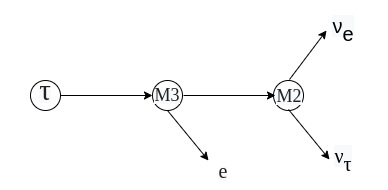
\includegraphics[width=14cm]{tauola_3body_phase_space.drawio.png}


\[AMS1 = M_{2,min} = m_{\nu_\tau}^2 \]
\[AMS2 = M_{2,max} = (M_{3} - m_e)^2\]

Flat Phase Spcae \\

\[AM2SQ = M_2^2 = M_{2,min} + U \times M_{2,max}  = m_{\nu_\tau}^2 + U \times (M_{3} - m_e)^2 \]


\[PHSPAC = \frac{1}{0.7 \times 2^{11} \pi^5} \times \Big((M_{3} - m_e)^2 - m_{\nu_\tau}^2\Big)\]

Neutrino rest frame \\

\[E_{\nu_\tau} = \frac{ M_2^2 + m_{\nu_\tau}^2 }{2M_2}\]
\[E_{\nu_e} = \frac{ M_2^2 - m_{\nu_\tau}^2 }{2M_2} \]


\[|p_{\nu_\tau}| = \sqrt{E_{\nu_\tau} - m_{\nu_\tau}^2 }\]

\[PHSPAC = \frac{1}{0.7 \times 2^{11} \pi^5} \times \Big((M_{3} - m_e)^2 - m_{\nu_\tau}^2\Big)\times 4\pi \times \frac{2|p_{\nu_\tau}|}{M_2}\]


The generation of random direction to fix the $\nu_\tau$ is shown after the following part


Intermediate particle four momentum - 

\[PR(4) = E_{2} =  \frac{1}{2M_3}(M_3^2 + M_2^2 - m_e^2)\]  

\[PR(3) = p_{2} = \sqrt{E_{2}^2 - M_2^2}\]

The electron momentum

\[QP(4) = E_e = \frac{1}{2M_3}(M_3^2 + m_e^2 - M_2^2)\]
\[QP(3) = p_e = -PR(3)\]

\[PHSPAC = \frac{1}{0.7 \times 2^{11} \pi^5} \times \Big((M_{3} - m_e)^2 - m_{\nu_\tau}^2\Big)\times 4\pi \times \frac{2|p_{\nu_\tau}|}{M_2} \times 4\pi \times \frac{2|p_2|}{M_3}\]


\subsubsection{Generate $\nu_\tau$ and $\nu_e$ momenta in random direction}

The $\nu_\tau$ and $\nu_e$ momenta direction is randomly generated and made both momenta opposite, which corresponsd to XN and XA.


\[EXE= e^\eta = \frac{PR(4)+PR(3)}{M_2} = \frac{E_2+p_2}{M_2}\]

Boost both XA and XN to rest frame of $M_2$. 


{\color{red} If there is radiative corrections then }\\

\[EPS =4 \Big(\frac{m_e}{m_\tau}\Big)^2\]
\[XL1 = log\Bigg(  \frac{2+4  (\frac{m_e}{m_\tau})^2 }{4  (\frac{m_e}{m_\tau})^2}       \Bigg)\]

\[XL0 = log\Bigg( 4 \Big(\frac{m_e}{m_\tau}\Big)^2 \Bigg)\]

\[ETA = exp\Bigg(log\Bigg( 4 \Big(\frac{m_e}{m_\tau}\Big)^2 \Bigg) + U \times log\Bigg(  \frac{2+4  (\frac{m_e}{m_\tau})^2 }{4  (\frac{m_e}{m_\tau})^2}       \Bigg)\Bigg)\]

\[CTHET = 1+EPS-ETA\]
\[THET =ACOS(CTHET) \]

Not sure it will generate spherical distribution

\[PHSPAC  = \frac{1}{0.7 \times 2^{11} \pi^5} \times \Big((M_{3} - m_e)^2 - m_{\nu_\tau}^2\Big)\times 4\pi \times \frac{2|p_{\nu_\tau}|}{M_2} \times 4\pi \times \frac{2|p_2|}{M_3} \times \frac{1}{2} log\Bigg(  \frac{2+4  (\frac{m_e}{m_\tau})^2 }{4  (\frac{m_e}{m_\tau})^2}       \Bigg) \times ETA\]

Rotate $\nu_\tau$, $\nu_e$, e, $M_2$ randomly. But all these particles has to have same random rotation.

And finally define the $\tau$ rest frame momenta and $\gamma$ momenta.

\[E_\tau = \frac{1}{2m_\tau}(m_\tau^2 + M_3^2)\]

\[p_\tau = \sqrt{E_\tau^2 - M_3^2}\]

\[\phi  = \frac{1}{0.7 \times 2^{11} \pi^5} \times \Big((M_{3} - m_e)^2 - m_{\nu_\tau}^2\Big)\times 4\pi \times \frac{2|p_{\nu_\tau}|}{M_2} \times 4\pi \times \frac{2|p_2|}{M_3} \times \frac{1}{2} log\Bigg(  \frac{2+4  (\frac{m_e}{m_\tau})^2 }{4  (\frac{m_e}{m_\tau})^2}       \Bigg) \times ETA \times 4\pi \times \frac{2|p_\tau|}{M_\tau}\]


Make the $\gamma$ momentum the opposite of tau momentum PAA.

{\color{red} If there is no radiative corrections then }\\

Rotate $\nu_\tau$, $\nu_e$, e, $M_2$ randomly. But all these particles has to have same random rotation. And finally define the $\tau$ rest frame momenta to be zero. Also no $\gamma$ emitted.


Call for DAMPRY to calculate the matrix element


\subsection{DAM4PI}
\textbf{SUBROUTINE DAM4PI(MNUM,PT,PN,PIM1,PIM2,PIM3,PIM4,AMPLIT,HV)}     Line 3732\\

The \textbf{MNUM} integer identifies the decay mode. \\

PT(4): 4-momentum of the tau lepton.\\

PN(4): 4-momentum of the neutrino. \\

PIM1(4), PIM2(4), PIM3(4), PIM4(4): 4-momenta of the four pions. \\

AMPLIT: Output variable storing the computed matrix element.\\

HV(4): Output polarimeter vector related to spin effects.\\



EXTERNAL FORM1,FORM2,FORM3,FORM4,FORM5   -- These external functions compute hadronic form factors.\\


If IME=2, choose the standard matrix element calculation.\\


The decay mode MNUM=1 or 2 selects a specific hadronic current model.\\

If IFBABAR=1, use the BABAR experimental model.\\

This is used in BABAR to simulate \textbf{tau decays} and compare with experimental data.


The code is organized in such a way that the hadronic currents provided by a sperate model is seprated from the part where we calculate the matrix element. 

\subsubsection{Hadronic Current \( J^\mu \) in Tau Decay}


One of the main difficulties in the study of four pion production is caused by the
existence of different intermediate states via which the final state could be produced, such
as \(\omega \pi\), \(\rho \sigma\), \(a_1(1260)\pi\), \(h_1(1170)\), \(\rho^+ \rho^- \), \(a_2(1320)\pi\), \(\pi(1300)\pi\).


In tau decays into multiple pions, the hadronic current \( J^\mu \) describes the interaction of hadrons (pions) with the weak interaction. Mathematically, the total hadronic current can be expressed as:

\begin{equation}
J^\mu = \sum_i C_i H_i^\mu
\end{equation}

where:
\begin{itemize}
    \item \( H_i^\mu \) are different hadronic contributions (vector and axial-vector components),
    \item \( C_i \) are their corresponding coefficients.
\end{itemize}

The subroutine computes these components based on the \textbf{four-momenta} of pions and resonance propagators.

\subsubsection{Resonance Contributions and Breit-Wigner Propagators}

A \textbf{Breit-Wigner function} is used to model resonances like the \(\rho\), \(\omega\), and \( a_1 \) mesons. The general form of a Breit-Wigner propagator is:

\begin{equation}
BW(M, \Gamma, s) = \frac{1}{s - M^2 + i M \Gamma}
\end{equation}

where:
\begin{itemize}
    \item \( M \) is the resonance mass,
    \item \( \Gamma \) is the resonance width,
    \item \( s \) is the invariant mass squared of the intermediate state.
\end{itemize}

For example, in the subroutine:
\begin{verbatim}
BWIGN(A,XM,XG) = 1.0 / CMPLX(A - XM**2, XM * XG)
\end{verbatim}
represents a Breit-Wigner propagator.

\subsubsection{Resonance Contributions}
\begin{itemize}
    \item The \(\rho\) meson dominates the \( 4\pi \) system, with form factors modifying its contribution.
    \item The \(\omega\) meson contributes through interference terms.
    \item The \( a_1(1260) \) resonance contributes to the axial-vector component.
\end{itemize}

\subsubsection{Kinematic Invariants and Scalar Products}

In the subroutine, the four-momentum scalar products and kinematic invariants are computed to construct the current:

\begin{equation}
P_i \cdot P_j = P_i^0 P_j^0 - P_i^1 P_j^1 - P_i^2 P_j^2 - P_i^3 P_j^3
\end{equation}

which are used to define:
\begin{itemize}
    \item \( QMP_k \) (invariant mass squared for three-pion subsystems),
    \item \( PS_{ij} \) (invariant mass squared for two-pion subsystems),
    \item \( PD_{ijk} \) (scalar triple products).
\end{itemize}

For example:

\begin{equation}
QMP1 = (P_2 + P_3 + P_4)^2
\end{equation}

where \( P_2, P_3, P_4 \) are the four-momenta of three pions.

\subsubsection{Structure of the Hadronic Current}

The \textbf{hadronic current} is constructed from:
\begin{itemize}
    \item \textbf{Vector form factors} (\( F_{\rho} \), \( F_{\omega} \), etc.).
    \item \textbf{Axial-vector contributions} (\( F_{a_1} \)).
    \item \textbf{Symmetric and antisymmetric tensor structures} for spin interactions.
\end{itemize}

The final current is a linear combination of these contributions:

\begin{equation}
H^\mu = C_1 \sum_{i<j} T_{ij} + C_2 \sum_{i<j<k} S_{ijk}
\end{equation}

where:
\begin{itemize}
    \item \( T_{ij} \) are \textbf{vector meson contributions} (like \( \rho \) propagators),
    \item \( S_{ijk} \) are \textbf{axial-vector meson contributions} (like \( a_1 \) propagators).
\end{itemize}

In the code:

\begin{verbatim}
T243 = BWIGA1(QMP2) * FPIKM(SQRT(PS43),AMPI,AMPI) * GAMMA1
\end{verbatim}

This corresponds to a \textbf{Breit-Wigner propagator of the \( a_1 \)}, multiplied by a \textbf{form factor} \( F_{\pi K} \) and a coupling \( \Gamma_1 \).

Similarly:

\begin{verbatim}
S2413 = FRHO4(SQRT(PS24),AMPI,AMPI) * GAMMA2
\end{verbatim}

This represents a \textbf{rho-meson contribution}.

\subsubsection{Final Hadronic Current and Amplitude}

The \textbf{final amplitude} for the tau decay is given by:

\begin{equation}
\mathcal{M} \propto J^\mu W_{\mu\nu} L^\nu
\end{equation}

where:
\begin{itemize}
    \item \( J^\mu \) is the hadronic current,
    \item \( W_{\mu\nu} \) is the hadronic tensor,
    \item \( L^\nu \) is the leptonic current.
\end{itemize}

The subroutine constructs \( J^\mu \) by computing all these terms, ensuring conservation of the weak current.


The subroutine implements the \textbf{hadronic current} for the \(\tau \to 4\pi \nu_\tau\) decay, using:
\begin{itemize}
    \item \textbf{Kinematic invariants} to construct momenta scalar products.
    \item \textbf{Breit-Wigner propagators} for resonances (\( \rho, \omega, a_1 \)).
    \item \textbf{Form factors and couplings} for weak interactions.
    \item \textbf{Tensor structures} to encode spin interactions.
\end{itemize}


-----------------------------------------------------------------------------------------------------------------\\

\subsubsection{\texttt{CURR\_KARLS}}

The subroutine \texttt{CURR\_KARLS} computes the hadronic current \( J^\mu \) for different final-state pion configurations in tau decays. It takes as input the four-momenta of four pions and produces the complex hadronic current.


\textbf{Inputs:}
\begin{itemize}
    \item \( PIM1^\mu, PIM2^\mu, PIM3^\mu, PIM4^\mu \) (four-momenta of pions)
    \item \( MNUM \) (integer identifying the pion configuration)
\end{itemize}

\textbf{Output:}
\begin{itemize}
    \item \( HADCUR^\mu \) (complex hadronic current)
\end{itemize}

\subsubsection{Four-Momentum Assignment}

For each pion configuration (\( MNUM = 1 \) or \( MNUM = 2 \)), the subroutine assigns four-momentum components:

\begin{equation}
    Q_i^\mu = (E_i, p_i^1, p_i^2, p_i^3), \quad i = 1,2,3,4
\end{equation}

where:
\begin{itemize}
    \item \( Q_1^\mu \) corresponds to \( PIM1^\mu \),
    \item \( Q_2^\mu \) corresponds to \( PIM2^\mu \),
    \item \( Q_3^\mu \) corresponds to \( PIM3^\mu \),
    \item \( Q_4^\mu \) corresponds to \( PIM4^\mu \).
\end{itemize}

\subsubsection{Invariant Mass Squared Calculation}

The invariant mass squared of the four-pion system is computed as:

\begin{equation}
    s = QQ2 = \left( \sum_{i=1}^{4} Q_i^0 \right)^2 - \sum_{j=1}^{3} \left( \sum_{i=1}^{4} Q_i^j \right)^2
\end{equation}

where:
\begin{itemize}
    \item \( Q_i^0 \) is the energy component of \( Q_i^\mu \),
    \item \( Q_i^j \) are the spatial components.
\end{itemize}

\subsubsection{Hadronic Current Calculation}

Depending on \( MNUM \), the subroutine calls different hadronic current models:
\begin{itemize}
    \item For \( MNUM = 1 \), the routine calls:
    \begin{equation}
        H^\mu = \text{HAD4}(s, Q_1, Q_2, Q_4, Q_3)
    \end{equation}
    which rearranges pion indices to match the TAUOLA conventions.
    \item For \( MNUM = 2 \), the routine calls:
    \begin{equation}
        H^\mu = \text{HAD3}(s, Q_1, Q_2, Q_3, Q_4)
    \end{equation}
\end{itemize}

\subsubsection{Final Hadronic Current Output}

The computed hadronic current \( H^\mu \) is stored in:

\begin{equation}
    HADCUR^\mu = (HADR^1, HADR^2, HADR^3, HADR^4)
\end{equation}

where:
\begin{itemize}
    \item \( HADCUR^4 = HADR^1 \) (time component),
    \item \( HADCUR^i = HADR^{i+1} \) for \( i = 1,2,3 \) (spatial components).
\end{itemize}


The subroutine computes the hadronic current using:
\begin{itemize}
    \item Four-momentum assignments for pions.
    \item Invariant mass squared \( QQ2 \).
    \item Calls to resonance-based hadronic current models (\texttt{HAD3}, \texttt{HAD4}).
    \item Reordering of pions to match TAUOLA conventions.
\end{itemize}

This is used in tau decay simulations for hadronic final states.


-----------------------------------------------------------------------------------------------------------------\\


\subsubsection{CURR$\_$BINP}
The hadronic current for the process $\tau^+ \to \pi A_1 (\rho + \sigma) \to 4\pi$ is computed using a sum over various contributions. This is based on the reference \cite{hep-ph/0201149}.

The hadronic final state in the semi leptonic decay of the tau lepton predominantly forms through the intermediate resonances, specifically:
\begin{itemize}
\item \(a_1\)(1260) meson decaying into three pion.
\item $\omega $ meson decaying into three pions.
\end{itemize}


The $a_1$ meson decay mode consist of two dominant decay modes, 
\begin{itemize}
\item \(a_1 \to \rho \pi \to 3\pi\)
\item \(a_1 \to \sigma \pi \to 3\pi\)
\end{itemize}

This hadronic current receives an additional contribution from the $\omega$ resonance. 
\begin{itemize}
\item \(\omega \to \rho \pi \to 3\pi\)
\end{itemize}
%%%%%%%%%%%%%%%%%%%%%%%%%%%%%%%%%%%%%%%%%%%%%%%%%%%%%%%%%%%%%%%
\subsubsection*{Derivation of the Hadronic Current for $\tau^+ \to \bar{\nu}_{\tau} \pi^+ \pi^0 \pi^0$}

The hadronic current for the decay channel $\tau^+ \to \bar{\nu}_{\tau} \pi^+ \pi^0 \pi^0$ follows from the chiral Lagrangian approach or Resonance Chiral Theory (R$\chi$T). 

\subsubsection*{Hadronic Current Structure}
The hadronic current $J^\mu$ describes the transition of the axial-vector resonance $a_1^+$ into the three-pion final state. It incorporates contributions from intermediate resonances such as the $\rho$ meson and the $\sigma$ meson. The hadronic current is parameterized as:

\begin{equation}
J^\mu_{a_1 \to \rho \pi} = G_{\pi^+\pi^0\pi^0\pi^0} (Q^2) \sum_{\text{permutations}} t_1^\mu,
\end{equation}

\begin{equation}
J^\mu_{a_1 \to \sigma \pi} = G_{\pi^+\pi^0\pi^0\pi^0} (Q^2) \sum_{\text{permutations}} t_2^\mu,
\end{equation}

where $G_{\pi^+\pi^0\pi^0\pi^0} (Q^2)$ is some function, which we find by fitting $4\pi$ invariant mass distribution, and the terms $t_1^\mu$ and $t_2^\mu$ describe different resonance-mediated contributions.\\




We consider two important decay channels of the $a_1$ meson leading to a three-pion final state:
\[
a_1 \to \rho \pi \to 3\pi, \quad a_1 \to \sigma \pi \to 3\pi.
\]
Taking into account the quantum numbers of the pion and the $a_1$-meson, the matrix elements for the processes
\[
\tilde{\rho}(P) \to a_1(q)\pi(p), \quad a_1(q) \to \rho(P')\pi(p), \quad a_1(q) \to \sigma(P')\pi(p)
\]
can be written as:
\begin{align}
    T(\tilde{\rho} \to a_1 \pi) &= F_{\tilde{\rho} a_1 \pi} \epsilon^{abc} (P_{\mu} \tilde{e}^{a}_{\nu} - P_{\nu} \tilde{e}^{a}_{\mu}) q_{\mu} A_{\nu}^{b*} \phi^{c*}, \\
    T(a_1 \to \rho \pi) &= F_{a_1 \rho \pi} \epsilon^{abc} q_{\mu} A_{\nu}^{a} (P'_{\mu} e_{\nu}^{b*} - P'_{\nu} e_{\mu}^{b*}) \phi^{c*}, \\
    T(a_1 \to \sigma \pi) &= F_{a_1 \sigma \pi} (q_{\mu} A_{\nu}^{a} - q_{\nu} A_{\mu}^{a}) P'_{\mu} P'_{\nu} \phi^{a*},
\end{align}
where $a, b, c$ are isospin indices, $A_{\mu}^{a}$ and $e_{\mu}^{a}$ are the polarization vectors of $a_1$ and $\rho$ mesons respectively, and $\phi^b$ represents the pion wave function. The factors $F_{\tilde{\rho} a_1 \pi}$, $F_{a_1 \rho \pi}$, and $F_{a_1 \sigma \pi}$ are form factors that depend on the kinematics of the process.

Furthermore, the transitions of $\rho$ and $\sigma$ mesons to pions are given by:
\begin{align}
    T(\rho \to \pi \pi) &= F_{\rho \pi \pi} \epsilon^{abc} e_{\mu}^{a} (p_{\mu}^{(b)} - p_{\mu}^{(c)}) \phi^{b*} \phi^{c*}, \\
    T(\sigma \to \pi \pi) &= F_{\sigma \pi \pi} \phi^{a k} \phi^{a k*},
\end{align}
where $p_{\mu}^{(b)}$ and $p_{\mu}^{(c)}$ are the four-momenta of the corresponding pions.

%%%%%%%%%%%%%%%%%%%%%%%%%%%%%%%%%%%%%%%%%%%%%%%%%%%%%%%%%%%%%%%%


\section{Introduction}
The quantum numbers of the $a_1(1260)$ resonance are $I^G J^{PC} = 1^{-}1^{++}$. Considering the quantum numbers of the pion, we can derive the matrix elements for the following processes:
\begin{equation}
\tilde{\rho}(P) \to a_1(q)\pi(p),
\end{equation}
and
\begin{equation}
a_1(q) \to \rho(P')\pi(p).
\end{equation}

\section{Matrix Element for $\tilde{\rho} \to a_1\pi$}
The transition amplitude for the process $\tilde{\rho} \to a_1\pi$ is given by:
\begin{equation}
T(\tilde{\rho} \to a_1\pi) = F_{\tilde{\rho} a_1 \pi} \varepsilon^{3ab} (P_\mu \tilde{e}\nu - P\nu \tilde{e}\mu) q\mu A^a_\nu \phi^{b*},
\end{equation}
where:
\begin{itemize}
\item $F_{\tilde{\rho} a_1 \pi}$ is the form factor,
\item $\varepsilon^{3ab}$ is the antisymmetric Levi-Civita symbol in isospin space,
\item $P_\mu, P_\nu$ are the 4-momenta of the $\tilde{\rho}$ meson,
\item $\tilde{e}\mu$ is the polarization vector of the $\tilde{\rho}$ meson,
\item $q\mu$ is the 4-momentum of the $a_1$ meson,
\item $A^a_\nu$ is the polarization vector of the $a_1$ meson,
\item $\phi^{b*}$ represents the pion wave function.
\end{itemize}

\section{Matrix Element for $a_1 \to \rho\pi$}
Similarly, the matrix element for the decay $a_1 \to \rho\pi$ is given by:
\begin{equation}
T(a_1 \to \rho\pi) = F_{a_1 \rho \pi} \varepsilon^{abc} q_\mu A^a_\nu (P'\mu e^{b*}\nu - P'\nu e^{b*}\mu) \phi^{c*},
\end{equation}
where:
\begin{itemize}
\item $F_{a_1 \rho \pi}$ is another form factor,
\item $e^{b*}\mu$ is the polarization vector of the $\rho$ meson,
\item $P'\mu$ is the 4-momentum of the $\rho$ meson.
\end{itemize}

\section{Matrix Element for $\rho \to \pi\pi$}
Finally, the transition matrix element for the decay $\rho \to \pi\pi$ reads:
\begin{equation}
T(\rho \to \pi\pi) = F_{\rho \pi \pi} \varepsilon^{abc} e^a_\mu (p^{(b)}\mu - p^{(c)}\mu) \phi^{b*} \phi^{c*},
\end{equation}
where $p^{(b)}\mu$ and $p^{(c)}\mu$ are the 4-momenta of the two pions.

\section{Helicity Considerations}
Due to helicity conservation, only the transverse space components of the 4-vector $\tilde{e}\mu$ are nonzero. We denote them as $\tilde{e}\perp$. For unpolarized electrons and positrons, the squared matrix element for the process $\tilde{\rho} \to 4\pi$ takes the form:
\begin{equation}
|T|^2 = |\mathbf{J}_\perp|^2.
\end{equation}

\section{Conclusion}
The matrix elements derived here provide the necessary formalism to describe the decay channels involving the $a_1(1260)$ resonance and its contribution to multi-pion final states. The form factors $F_{\tilde{\rho} a_1 \pi}, F_{a_1 \rho \pi},$ and $F_{\rho \pi \pi}$ encapsulate the dynamics of the interactions and introduce theoretical uncertainties in the model.

%%%%%%%%%%%%%%%%%%%%%%%%%%%%%%%%%%%%%%%%%%%%%%%%%%%%%%%%%%%%%%%%%

\subsubsection*{Four-Vector Definitions}
The explicit forms of the four-vectors $t_1^\mu$ and $t_2^\mu$ are given by:
\begin{equation}
t_1^\mu(q_1, q_2, q_3, q_4) = \frac{F^2_{a_1} (Q - q_1)}{D_{a_1}(Q - q_1) D_\rho(q_3 + q_4)} \Big[ (Q \cdot (Q - q_1)) (q_4^\mu (Q - q_1) \cdot q_3 - q_3^\mu (Q - q_1) \cdot q_4)
\end{equation}
\begin{equation}
+ (Q^\mu - q_1^\mu)((Q - q_4)(q_1 \cdot q_3) - (Q \cdot q_3)(q_4 \cdot q_1)) \Big],
\end{equation}
\begin{equation}
t_2^\mu(q_1, q_2, q_3, q_4) = \frac{zF^2_{a_1} (Q - q_1)}{D_{a_1}(Q - q_1) D_\sigma(q_3 + q_4)} \Big[ q_2^\mu Q \cdot (Q - q_1) - (Q^\mu (Q - q_1) \cdot q_2 + (Q - q_1)^2 q_2^\mu) \Big].
\end{equation}

\subsubsection*{Sign Differences in Equations (14) and (15)}
The sign differences arise because:
\begin{itemize}
\item The $a_1 \to \rho\pi$ transition is mediated by the vector meson $\rho$, which follows a symmetric contribution of permutations.
\item The $a_1 \to \sigma\pi$ transition involves the scalar meson $\sigma$, leading to an asymmetric term due to interference effects.
\item The interference terms in the $\sigma\pi$ case require certain terms to appear with a negative sign, ensuring the correct Bose symmetry of the final state.
\end{itemize}

The structure of the hadronic current is dictated by the intermediate resonances and their symmetry properties. The $\rho$-mediated terms are symmetric, while the $\sigma$-mediated terms include antisymmetric contributions, leading to sign differences in Equations (14) and (15).




%%%%%%%%%%%%%%%%%%%%%%%%%%%%%%%%%%%%%%%%%%%%%%%%%%%%%%%%%%%%%%%%
\subsubsection{Four-Momentum Definition}
The four-momentum of the pions involved in the decay are denoted as:
\begin{equation}
p_1^\mu, p_2^\mu, p_3^\mu, p_4^\mu
\end{equation}
and the total four-momentum is given by:
\begin{equation}
p_a^\mu = p_1^\mu + p_2^\mu + p_3^\mu + p_4^\mu.
\end{equation}

The invariant mass squared is:
\begin{equation}
s = p_a^\mu p_{a\mu}.
\end{equation}



\subsubsection{Some initialization}

\begin{align*}
&m_\rho = 0.7761\,GeV\\
&\Gamma_\rho = 0.1445\,GeV
\end{align*}

\subsubsection{\texttt{LATA}}

The subroutine \texttt{LATA} is responsible for converting the convention of a 4-vector representation between two different forms:
\begin{itemize}
    \item \((x, y, z, E)\) — used in \texttt{TAUOLA}
    \item \((E, x, y, z)\) — used in \texttt{BINP}
\end{itemize}
where:
\begin{itemize}
    \item \( E \) is the energy component.
    \item \( (x, y, z) \) are the spatial components of the 4-vector.
\end{itemize}

 
1. **Case \( \texttt{key} = 1 \) (Converting from \((x,y,z,E)\) to \((E,x,y,z)\))**  
   
2. **Case \( \texttt{key} \neq 1 \) (Converting from \((E,x,y,z)\) to \((x,y,z,E)\))**  
   
%%%%%%%%%%%%%%%%%%%%%%%%%%%%%%%%%%%%%%%%%%%%%%%%%%%

\subsubsection{\texttt{T1}}

The subroutine \texttt{T1} computes a matrix element for the process \( a1 \to \rho + \pi  \), based on Eq. (16) in \texttt{hep-ph/0201149}. It originates from the Novosibirsk code, specifically the \texttt{z\_a1rho} subroutine.
\begin{itemize}

\item Input Variables:\\
- \( p_1^\mu \) : 4-momentum of \( \pi^+ \).\\
- \( p_2^\mu , p_3^\mu, p_4^\mu \) : 4-momentum of \( \pi^0 \).\\
- \( z_{\text{vec}}^\mu \) : Computed vector output.

\item Definitions:
The total momentum of the system is computed as:
\[
p_a^\mu = p_1^\mu + p_2^\mu + p_3^\mu + p_4^\mu.
\]

\subsubsection{$\texttt{z\_drho(p1, p2)}$}

The function $\texttt{z\_drho(p1, p2)}$ computes the propagator of the $\rho$ meson based on the prescription given in Eq. (18) of hep-ph/0201149. The following steps describe its implementation:

\subsubsection{Computation of the Mandelstam Variable \( s \)}

The squared invariant mass $s$ of the system formed by the four-momenta $p_1$ and $p_2$ is computed as:
\begin{equation}
s = (E_1 + E_2)^2 - (\mathbf{p}_1 + \mathbf{p}_2)^2.
\end{equation}
In component form, this is:
\begin{equation}
s = (p_1^0 + p_2^0)^2 - (p_1^1 + p_2^1)^2 - (p_1^2 + p_2^2)^2 - (p_1^3 + p_2^3)^2.
\end{equation}

\subsubsection{Phase Space Factor \( g(s) \)}

The phase space factor $g(s)$ accounts for the available decay phase space:
\begin{equation}
g(s) = \sqrt{\max \left( \frac{(s - 4 m_{\pi}^2)^3}{s}, 0 \right)},
\end{equation}
where $m_{\pi}$ is the pion mass.

\subsubsection{Dynamical Width Contribution \( \Gamma_{\rho}(s) \)}

The function introduces a running width term $\Gamma_{\rho}(s)$:
\begin{equation}
GamMas = \Gamma_{\rho} \cdot M_{\rho},
\end{equation}
where $M_{\rho}$ and $\Gamma_{\rho}$ are the mass and width of the $\rho$ meson.

\subsubsection{Propagator Calculation}

The $\rho$ meson propagator is given by:
\begin{equation}
z_{d\rho}(s) = \frac{s - M_{\rho}^2 - d_m(s) \Gamma_{\rho} M_{\rho} + i \Gamma_{\rho} M_{\rho} \frac{g(s)}{g(M_{\rho}^2)}}{M_{\rho}^2}.
\end{equation}
%%%%%%%%%%%%%%%%%%%%%%%%%%%%%%%%%%%%%%%%%%%%%%%%%%

The function \texttt{dm(s)} computes the mass correction to the rho propagator. The formula for \texttt{dm(s)} is:

\[
\text{dm}(s) = \frac{h_\rho(s) - h_\rho(M_\rho^2) - (s - M_\rho^2) \, \frac{d h_\rho}{d s}(m^2)}{g(M_\rho^2)}
\]

where:
\begin{itemize}
    \item \( s \) is the Mandelstam variable (the square of the energy in the center-of-mass frame of the system).
    \item \( h_\rho(s) \) is a function related to the rho meson propagator.
    \item \( \frac{d h_\rho}{d s}(s) \) is the derivative of \( h_\rho(s) \) with respect to \( s \).
    \item \( g(M_\rho^2) \) is a normalization factor that depends on the mass of the rho meson.
\end{itemize}

\begin{align*}
& g(M_\rho^2) = M_\rho^2 \left( \sqrt{1 - \frac{(2 m_{\pi})^2}{M_\rho^2}} \right)^3
\end{align*}

\subsubsection*{Function \texttt{hrho(s)}}

The function \texttt{hrho(s)} computes the rho meson propagator term. The formula for \( h_\rho(s) \) is:

For \( s = 0 \):
\[
h_\rho(s) = - \frac{2 \cdot 4 \cdot m_\pi^2}{\pi}
\]

For \( s \neq 0 \), the formula is:
\[
h_\rho(s) = \frac{y \cdot \ln\left(\frac{1 + y}{1 - y}\right) \cdot (s - 4m_\pi^2)}{\pi}
\]
where:
\[
y = \sqrt{1 - \frac{4m_\pi^2}{s}}
\]

\subsubsection*{Function \texttt{dhrho(s)}}

The function \texttt{dhrho(s)} computes the derivative of the propagator term \( h_\rho(s) \), denoted \( \frac{d h_\rho}{d s}(s) \). The formula for the derivative is:

\[
\frac{d h_\rho}{d s}(s) = \frac{w + \left( \frac{dy}{ds} a + 1 \right) y^2}{\pi}
\]
where:
\[
w = y \cdot a, \quad a = \ln\left(\frac{1 + y}{1 - y}\right)
\]
and
\[
\frac{dy}{ds} = \frac{4 m_\pi^2}{2 s y}
\]

This gives the rate of change of the propagator term with respect to \( s \).


%%%%%%%%%%%%%%%%%%%%%%%%%%%%%%%%%%%%%%%%%%%%%%%%%%
The final normalization is:
\begin{equation}
z_{d\rho}(s) \to \frac{z_{d\rho}(s)}{1 + \frac{\Gamma_{\rho}}{M_{\rho}} d_m(0)}.
\end{equation}

This function calculates the denominator of the $\rho$ meson propagator, which is an essential component in describing its contribution to the scattering amplitude. It ensures the proper behavior of the $\rho$ resonance by incorporating an energy-dependent width and phase-space factor.




The squared momentum transfer is given by:
\[
s_a = (p_a^0 - p_1^0)^2 - (p_a^1 - p_1^1)^2 - (p_a^2 - p_1^2)^2 - (p_a^3 - p_1^3)^2.
\]
The function \( Z_{\rho} \) is obtained from the subroutine \texttt{z\_drho}, and the function \( Z_{a_1} \) is obtained from the subroutine \texttt{z\_da1}:
\[
Z_{\rho} = z_{\text{drho}}(p_3, p_4), \quad Z_{a_1} = z_{\text{da1}}(s_a).
\]

The subroutine \texttt{z\_da1} calculates the A1 propagator, which describes the interaction between pions and the A1 resonance. This propagator is based on an equation from the paper \texttt{hep-ph/0201149} (see Eq. (18) and internal notes). 

\subsubsection*{Variables and Parameters in z\_da1}
\begin{itemize}
  \item \texttt{AMass\_A} - The mass of the A1 resonance.
  \item \texttt{Gamma\_A} - The width of the A1 resonance.
  \item \texttt{Scale\_A} - A scale factor for the A1 resonance.
  \item \texttt{DWave\_A} - A complex variable that contains the values for the A1 propagator in real and imaginary parts.
  \item \texttt{sa\_q} - Input variable representing the q-momentum, used in the resonance width calculation.
  \item \texttt{pm} - A parameter representing the resonance width at the given momentum.
  \item \texttt{pm0} - The normalization width of the resonance.
  \item \texttt{gma1} - The width of the A1 resonance divided by its mass.
  \item \texttt{ama1} - The square of the A1 mass.
\end{itemize}

The code is structured as follows:

1. The subroutine first defines initial values for the A1 mass, width, scale, and the complex wave function for the A1 resonance.

\[
\texttt{Gamma\_A} = 0.45 \quad \text{(Width of A1)}
\]
\[
\texttt{AMass\_A} = 1.23 \quad \text{(Mass of A1)}
\]
\[
\texttt{Scale\_A} = 1.2 \quad \text{(Scale for A1)}
\]
\[
\texttt{DWave\_A} = (1.269, 0.591) \quad \text{(Complex values for A1 propagator)}
\]

2. If \texttt{ia1f} is zero, the code computes the resonance width using a function \texttt{gma1v}.

\[
\texttt{gma1} = \frac{\texttt{Gamma\_A}}{\texttt{AMass\_A}} \quad \text{(Resonance width normalized by mass)}
\]

3. The variable \texttt{pm} is calculated using the function \texttt{gma1v(sa\_q)}, which provides the resonance width as a function of the momentum:

\[
\texttt{pm} = \texttt{gma1v(sa\_q)} \quad \text{(Resonance width for the given momentum)}
\]

4. The propagator is then computed as a complex number:

\[
\texttt{z\_da1} = \texttt{DCMPLX}\left( \frac{\texttt{sa\_q}}{\texttt{ama1}} - 1.0, \frac{\texttt{gma1} \cdot \texttt{pm}}{\texttt{pm0}} \right)
\]

where \(\texttt{DCMPLX}\) creates a complex number with the real part \(\frac{\texttt{sa\_q}}{\texttt{ama1}} - 1.0\) and the imaginary part \(\frac{\texttt{gma1} \cdot \texttt{pm}}{\texttt{pm0}}\).

\subsubsection*{The Function \texttt{gma1v(X2)}}

This function calculates the width of the A1 resonance, which depends on the square of the mass, \(X^2\), and uses a table of precomputed values. The width is computed for different resonance decay channels, which include:

\[
\text{A1} \rightarrow \pi^+ \pi^- \pi^0 \quad \text{or} \quad \text{A1} \rightarrow 3 \pi^0
\]

This function utilizes pre-defined tables for the values of \(S\), \(\text{INTE}\), \(\text{INT\_ABS}\), \(\text{INT\_RE}\), and \(\text{INT\_IM}\), which contain the integration results for the respective decay channels.


The subroutine \texttt{z\_da1} calculates the complex A1 propagator based on the resonance parameters and momentum of the pions involved. The final result is a complex number, where the real and imaginary parts describe the amplitude of the A1 propagator.



\vspace{1cm}



The function \( f_s \) is computed as:
\[
f_s = \left( \frac{1 + \frac{M_{A}^2}{\text{Scale}_A}}{1 + \frac{s_a}{\text{Scale}_A}} \right)^2.
\]
The common factor \( f_{\text{com}} \) is defined as:
\[
f_{\text{com}} = \frac{f_s}{Z_{a_1} Z_{\rho}}.
\]

\item Scalar Products:
Several scalar products of the momenta are computed:
\[
\textbf{PPp1} = p_a \cdot p_a - p_a \cdot p_1,
\]
\[
\textbf{p4Pp1} = p_4 \cdot p_a - p_4 \cdot p_1,
\]
\[
\textbf{p3Pp1} = p_3 \cdot p_a - p_3 \cdot p_1,
\]
\[
\textbf{p3P} = p_3 \cdot p_a, \quad p4P = p_4 \cdot p_a,
\]
\[
\textbf{p1p3} = p_1 \cdot p_3, \quad p1p4 = p_1 \cdot p_4.
\]

\item Computation of \( z_{\text{vec}}^\mu \):
The output vector \( z_{\text{vec}}^\mu \) is calculated as:
\[
z_{\text{vec}}^\mu = f_{\text{com}} \left( \textbf{PPp1} \left( p_3^\mu \textbf{p4Pp1} - p_4^\mu \textbf{p3Pp1} \right) + (p_a^\mu - p_1^\mu) \left( \textbf{p3P} \cdot \textbf{p1p4} - \textbf{p4P} \cdot \textbf{p1p3} \right) \right).
\]

\item  Convention Change:
After computing \( z_{\text{vec}}^\mu \), the components are shifted to match the TAUOLA convention \((x,y,z,E)\). This is done by:
\[
z_{\text{ee}} = z_{\text{vec}}^1,
\]
\[
z_{\text{vec}}^i = z_{\text{vec}}^{i+1}, \quad i = 1,2,3,
\]
\[
z_{\text{vec}}^4 = z_{\text{ee}}.
\]



\end{itemize}
This ensures compatibility with TAUOLA's convention for 4-vectors.

%%%%%%%%%%%%%%%%%%%%%%%%%%%%%%%%%%%%%%%%%%%%%%%%%%%%%

\subsubsection{Hadronic Current Calculation}
The hadronic current is given by the sum over various contributions:
\begin{equation}
H^\mu = \sum_{i} J_i^\mu,
\end{equation}
where the individual contributions arise from different intermediate resonance channels (e.g., $\rho$, $\sigma$ exchange).

For $MNUM = 2$ (corresponding to $\tau^+ \to \pi^+ \pi^0 \pi^0 \pi^0$):
\begin{equation}
J^\mu = \sum_{\text{perms}} t_1(p_i, p_j, p_k, p_l) + \sum_{\text{perms}} t_2(p_i, p_j, p_k, p_l),
\end{equation}
where $t_1$ and $t_2$ correspond to different intermediate contributions via $\rho$ and $\sigma$.

For $MNUM = 1$ (corresponding to $\tau^+ \to \pi^+ \pi^- \pi^+ \pi^0$):
\begin{equation}
J^\mu = \sum_{\text{perms}} t_1(p_i, p_j, p_k, p_l) - \sum_{\text{perms}} t_2(p_i, p_j, p_k, p_l).
\end{equation}

The factor determining the strength of the current is:
\begin{equation}
F(s) = f(s) \cdot \frac{\sqrt{A \cdot \sqrt{s} - B}}{s \cdot M_{\rho}^{4}},
\end{equation}
where $f(s)$ is a resonance-dependent function.

For $MNUM = 1$:
\begin{equation}
F(s) = \text{fit}{a_1}(\sqrt{s}) \cdot 76.565 \cdot \frac{\sqrt{0.71709 \sqrt{s} - 0.27505}}{s \cdot M{\rho}^{4}}.
\end{equation}
For $MNUM = 2$:
\begin{equation}
F(s) = \text{fit}2(\sqrt{s}) \cdot 96.867 \cdot ZFA1TAB(s) \cdot \frac{\sqrt{0.70907 \sqrt{s} - 0.26413}}{s \cdot M{\rho}^{4}}.
\end{equation}


-----------------------------------------------------------------------------------------------------------------\\

\subsubsection{\texttt{CURR$\_$CLEO}}

The \texttt{CURR$\_$CLEO} subroutine computes the hadronic current for the four-pion final state in hadronic tau decays. It is based on models described in various theoretical studies \cite{fischer1980, decker1987, gellmann1962}. This document presents the mathematical formulation of the hadronic current using the Breit-Wigner resonance model and matrix element calculations.

\subsubsection{Hadronic Current}

The hadronic current is represented as a four-vector complex function $H^{\mu}$, which is constructed based on the momenta of the four pions involved:
\begin{equation}
H^{\mu} = \sum_{i=1}^{4} A_i P_i^{\mu},
\end{equation}
where $P_i^{\mu}$ are the four-momenta of the pions, and $A_i$ are complex coefficients that depend on resonance structures.

\subsubsection{Breit-Wigner Propagators}

The Breit-Wigner propagator is used to describe intermediate resonances in the decay process. It takes the form:
\begin{equation}
BW(s, M, \Gamma) = \frac{1}{s - M^2 + i M \Gamma},
\end{equation}
where:
\begin{itemize}
\item $s$ is the invariant mass squared of the resonance,
\item $M$ is the resonance mass,
\item $\Gamma$ is the decay width.
\end{itemize}
This propagator is used for intermediate $\rho$, $\omega$, and other vector mesons.

\subsubsection{Current Contributions from Resonances}

The hadronic current is constructed by summing over different resonance contributions:
\begin{equation}
H^{\mu} = \sum_{j} C_j BW(s_j, M_j, \Gamma_j) \times F_j(P_1, P_2, P_3, P_4),
\end{equation}
where $C_j$ are the complex amplitude coefficients and $F_j$ represents form factors constructed from pion momenta.

For instance, the $\rho$-mediated contributions take the form:
\begin{equation}
H^{\mu}{\rho} = (\lambda_0 + \lambda_1 BW(s, M\rho, \Gamma_\rho) + \lambda_2 BW(s, M_{\rho'}, \Gamma_{\rho'}) ) \cdot (P_1^{\mu} - P_2^{\mu}).
\end{equation}

Similarly, the $\omega$-mediated contributions involve additional Lorentz-invariant contractions of pion momenta:
\begin{equation}
H^{\mu}{\omega} = \alpha_0 + \alpha_1 BW(s, M\omega, \Gamma_\omega) \sum_{i,j} \epsilon^{\mu \nu \rho \sigma} P_i^{\nu} P_j^{\rho} P_k^{\sigma},
\end{equation}
where $\epsilon^{\mu \nu \rho \sigma}$ is the Levi-Civita symbol.



The \texttt{CURR$\_$CLEO} subroutine calculates the hadronic current using a combination of Breit-Wigner propagators, form factors, and Lorentz-invariant momentum contractions. The computed current is crucial for modeling hadronic tau decays in experimental and theoretical studies.


-----------------------------------------------------------------------------------------------------------------\\


\subsubsection*{Subroutine CLVEC Explanation}

The subroutine \texttt{CLVEC} calculates the "vector type" $\mathbf{PIV}$ based on the provided inputs: the neutrino momentum $\mathbf{P_N}$ and a complex vector $\mathbf{HJ}$. The calculation involves the following steps:

Let the 4-momentum of the neutrino be:
\[
\mathbf{P_N} = (P_N^1, P_N^2, P_N^3, P_N^4),
\]
where we assume that the neutrino momentum is along the $z$-axis, so:
\[
P_N^1 = P_N^2 = 0, \quad P_N^3 = P_N^z, \quad P_N^4 = P_N^t.
\]
The vector $\mathbf{HJ}$ is a complex 4-vector:
\[
\mathbf{HJ} = (H_J^1, H_J^2, H_J^3, H_J^4).
\]
The output vector is $\mathbf{PIV} = (PIV^1, PIV^2, PIV^3, PIV^4)$.

Step 1: Calculation of $HN$

The intermediate quantity $HN$ is computed as:
\[
HN = H_J^4 \cdot P_N^4 - H_J^3 \cdot P_N^3.
\]

Step 2: Calculation of $HH$

The value of $HH$ is computed as:
\[
HH = \text{Re}(H_J^4 \cdot \overline{H_J^4} - H_J^3 \cdot \overline{H_J^3} - H_J^2 \cdot \overline{H_J^2} - H_J^1 \cdot \overline{H_J^1}),
\]
where $\overline{H_J^i}$ represents the complex conjugate of $H_J^i$.

Step 3: Final Calculation of $\mathbf{PIV}$

The components of $\mathbf{PIV}$ are computed using:
\[
PIV^i = 4 \cdot \text{Re}(HN \cdot \overline{H_J^i}) - 2 \cdot HH \cdot P_N^i, \quad \text{for} \quad i = 1, 2, 3, 4.
\]

This gives the four components of $\mathbf{PIV}$, representing a vector in the same space as $\mathbf{HJ}$ and $\mathbf{P_N}$.

-----------------------------------------------------------------------------------------------------------------\\

\subsubsection*{Mathematical and Physics Explanation of the Subroutine \texttt{CLAXI}}

The subroutine \texttt{CLAXI} calculates the "axial type" \(\pi\)-vector \(\mathbf{PIA}\), which is a 4-vector. The inputs to the subroutine are:
- The neutrino momentum vector \(\mathbf{P_N} = (P_N^1, P_N^2, P_N^3, P_N^4)\),
- A complex 4-vector \(\mathbf{HJ} = (H_J^1, H_J^2, H_J^3, H_J^4)\).

The neutrino momentum \(\mathbf{P_N}\) is assumed to be aligned along the \(z\)-axis, i.e.:
\[
P_N^1 = P_N^2 = 0, \quad P_N^3 = P_N^z, \quad P_N^4 = P_N^t.
\]
The goal is to compute the axial \(\pi\)-vector \(\mathbf{PIA} = (PIA^1, PIA^2, PIA^3, PIA^4)\).

\subsubsection*{Steps in the Subroutine}

1. **Complex Conjugates:**

   First, the complex conjugates of the components of \(\mathbf{HJ}\) are computed:
   \[
   HJC^i = \overline{H_J^i}, \quad \text{for} \quad i = 1, 2, 3, 4.
   \]

2. **Computation of Determinants:**

   The subroutine uses a function \(\text{DET2}(i, j)\) to compute the imaginary part of the determinant of certain combinations of the components of \(\mathbf{HJ}\) and \(\mathbf{HJC}\). The function is defined as:
   \[
   \text{DET2}(i, j) = \text{Im}(HJC^i H_J^j - HJC^j H_J^i).
   \]

3. **Axial Vector Calculation:**

   The axial vector components \(PIA^1, PIA^2, PIA^3, PIA^4\) are then computed using the following formulas:
   \[
   PIA^1 = -2 P_N^3 \text{DET2}(2, 4) + 2 P_N^4 \text{DET2}(2, 3),
   \]
   \[
   PIA^2 = -2 P_N^4 \text{DET2}(1, 3) + 2 P_N^3 \text{DET2}(1, 4),
   \]
   \[
   PIA^3 = 2 P_N^4 \text{DET2}(1, 2),
   \]
   \[
   PIA^4 = 2 P_N^3 \text{DET2}(1, 2).
   \]

4. **Sign Assignment:**

   The sign of the components of \(\mathbf{PIA}\) is determined by the parameter \(\text{SIGN}\), which depends on the value of \(KTOM\) and the variable \(IDFF\). Specifically:
   \[
   \text{SIGN} = 
   \begin{cases}
   \frac{IDFF}{|IDFF|}, & \text{if } KTOM = 1 \text{ or } KTOM = -1, \\
   -\frac{IDFF}{|IDFF|}, & \text{if } KTOM = 2, \\
   \text{ERROR}, & \text{otherwise}.
   \end{cases}
   \]
   Finally, the components of \(\mathbf{PIA}\) are multiplied by the sign:
   \[
   PIA^i \rightarrow PIA^i \times \text{SIGN}, \quad \text{for } i = 1, 2, 3, 4.
   \]


-----------------------------------------------------------------------------------------------------------------\\
\subsubsection*{Mathematical Explanation of the Subroutine \texttt{CLNUT}}

The subroutine \texttt{CLNUT} calculates the contribution due to the neutrino mass in a given physical system, assuming the tau particle is at rest. The subroutine uses the input complex 4-vector \(\mathbf{HJ}\) and computes the result in the real 4-vector \(\mathbf{HV}\).

Inputs
- \(\mathbf{HJ} = (H_J^1, H_J^2, H_J^3, H_J^4)\), a complex 4-vector.
- \(\mathbf{P} = (P^1, P^2, P^3, P^4)\), a real 4-vector initialized with the values:
  \[
  P^1 = P^2 = P^3 = 0, \quad P^4 = 1.
  \]

Steps

1. **Call to Subroutine \texttt{CLAXI}:**
   The subroutine \texttt{CLNUT} calls another subroutine, \texttt{CLAXI}, which computes the axial vector \(\mathbf{PIA}\) based on the input \(\mathbf{HJ}\) and \(\mathbf{P}\). The result is stored in the real 4-vector \(\mathbf{HV}\), i.e.:
   \[
   \mathbf{HV} = \texttt{CLAXI}(\mathbf{HJ}, \mathbf{P}).
   \]

2. **Calculation of \(B\):**
   The value of \(B\) is computed as:
   \[
   B = \text{Re} \left( H_J^4 \, \text{Im}(H_J^4) - H_J^3 \, \text{Im}(H_J^3) - H_J^2 \, \text{Im}(H_J^2) - H_J^1 \, \text{Im}(H_J^1) \right),
   \]
   where \(\text{Re}\) and \(\text{Im}\) represent the real and imaginary parts, respectively, of the complex numbers.

 Output
- \(B\), a real scalar value representing the contribution from the neutrino mass.


-----------------------------------------------------------------------------------------------------------------\\

If IFBABAR=2, select between Karlsruhe (CURR$\_$KARLS) and Novosibirsk (CURR$\_$BINP) models.\\


If MNUM=1, sum contributions from different parameterizations.



If none of the above, use the CLEO experiment's hadronic current model.


\subsubsection{Computing the Matrix Element}

CALL CLVEC(HADCUR,PN,PIVEC)\\
CALL CLAXI(HADCUR,PN,PIAKS)\\
CALL CLNUT(HADCUR,BRAKM,HVM)\\

Compute vector, axial, and neutrino-related contributions using HADCUR.\\


\begin{align*}
&BRAK = (G_V^2 + G_A^2) p_\tau^\mu P_\mu  + 2G_VG_A p_\tau^\mu A_\mu + 2(G_V^2- G_A^2)m_{\nu^\tau}m_\tau BRAKM\\
&AMPLIT = (CCABIB* G_F)^2 \frac{BRAK}{2}
\end{align*}

\subsubsection{Computing the Polarimeter Vector}








\newpage
\section*{References}
\nocite{Siepe2024}
\printbibliography[heading=none]

\end{document}